



\section{Benchmark} 
\label{benchmark}
\noindent As shown in Fig.~\ref{fig: pipeline}, we introduce Domain-aware Diffusion (DaD) to narrow the image-level domain gap between synthetic pretraining datasets and real-world pedestrian retrieval datasets (target domain). 
The images generated by DaD form a new dataset, the Synthetic Domain-Aligned (SDA) dataset, augmented with image captions and region-phrase annotations. 
Multi-granularity Relation Alignment (MRA) is then employed to enforce fine-grained region-level alignment during person retrieval pretraining.
In this section, we will illustrate the specific details of DaD and SDA, while the MRA workflow is elaborated in Section \ref{method}.

\subsection{Domain-aware Diffusion} 
\noindent In this paper, we use one of the prevailing real-world person retrieval datasets, \ie, CUHK-PEDES, as the target domain dataset. Previous work~\cite{yang2023towards} leverages the texts from the target domain dataset as prompts to generate images by a Diffusion Model. The synthetic images are adopted to perform pretraining. 
To migrate the domain gap between the synthetic and real-world domain, we fine-tune a Text-to-Image Diffusion Model on the target domain dataset and represent the fine-tuned model as Domain-aware Diffusion (DaD). 
In ControlNet~\cite{zhang2023adding}, the pose of the generated image can be controlled by fine-tuning Stable Diffusion~\cite{sd15}. 
Inspired by this work, we control the style of the generated image through ControlNet for image-level domain adaptation. 
Specifically, Stable Diffusion~\cite{sd15} is essentially a U-Net~\cite{ronneberger2015u} consisting of an encoder (containing 12 blocks), a middle block, and a skip-connected decoder (containing 12 blocks). 
We utilize ControlNet to create trainable copies of the 12 encoding blocks and the single middle block of the Stable Diffusion model, as illustrated in Figure~\ref{fig: pipeline}. 
During model training, the original Stable Diffusion blocks remain frozen.
The outputs of these trainable copies are added to the corresponding 12 skip-connection blocks and the middle block of the Stable Diffusion model through zero convolutions. 
The zero convolution layer is a $1 \times 1$ convolution layer with both weight and bias initialized to zeros. 
Text prompts and diffusion timesteps are encoded using the CLIP text encoder~\cite{radford2021learning} and a positional encoding-based time encoder, respectively.
We take image-text pairs from the CUHK-PEDES training set as input, set the control condition as a full white image, and optimize the model using the $\mathcal{L}_{\text{MSE}}$ (Mean Square Error) loss shown in Figure~\ref{fig: pipeline}. 
The input image resolution is set to $384 \times 256$. 
We perform fine-tuning for 3 epochs to obtain a Domain-aware Diffusion model.
There are two main advantages:
(1) Compared with traditional style transfer models, \eg, CycleGAN~\cite{zhu2017unpaired}, we deploy a fine-tuned Text-to-Image Diffusion Model for domain adaptation. 
The diffusion model shows a strong and stable ability to generate images with high content consistency to text prompts. 
The fine-tuned diffusion model can greatly reduce the gap between the generated image and the source domain data, as shown in Fig.~\ref{fig: examples}.
(2) Using synthetic images will circumvent privacy issues. By utilizing DaD as an image generator, we can produce a diverse array of pedestrian images. This approach eliminates the need to expend manpower or resources on collecting real-world pedestrian images, thereby avoiding privacy concerns and reducing labor costs. 


\begin{figure*}[!t]
\centering
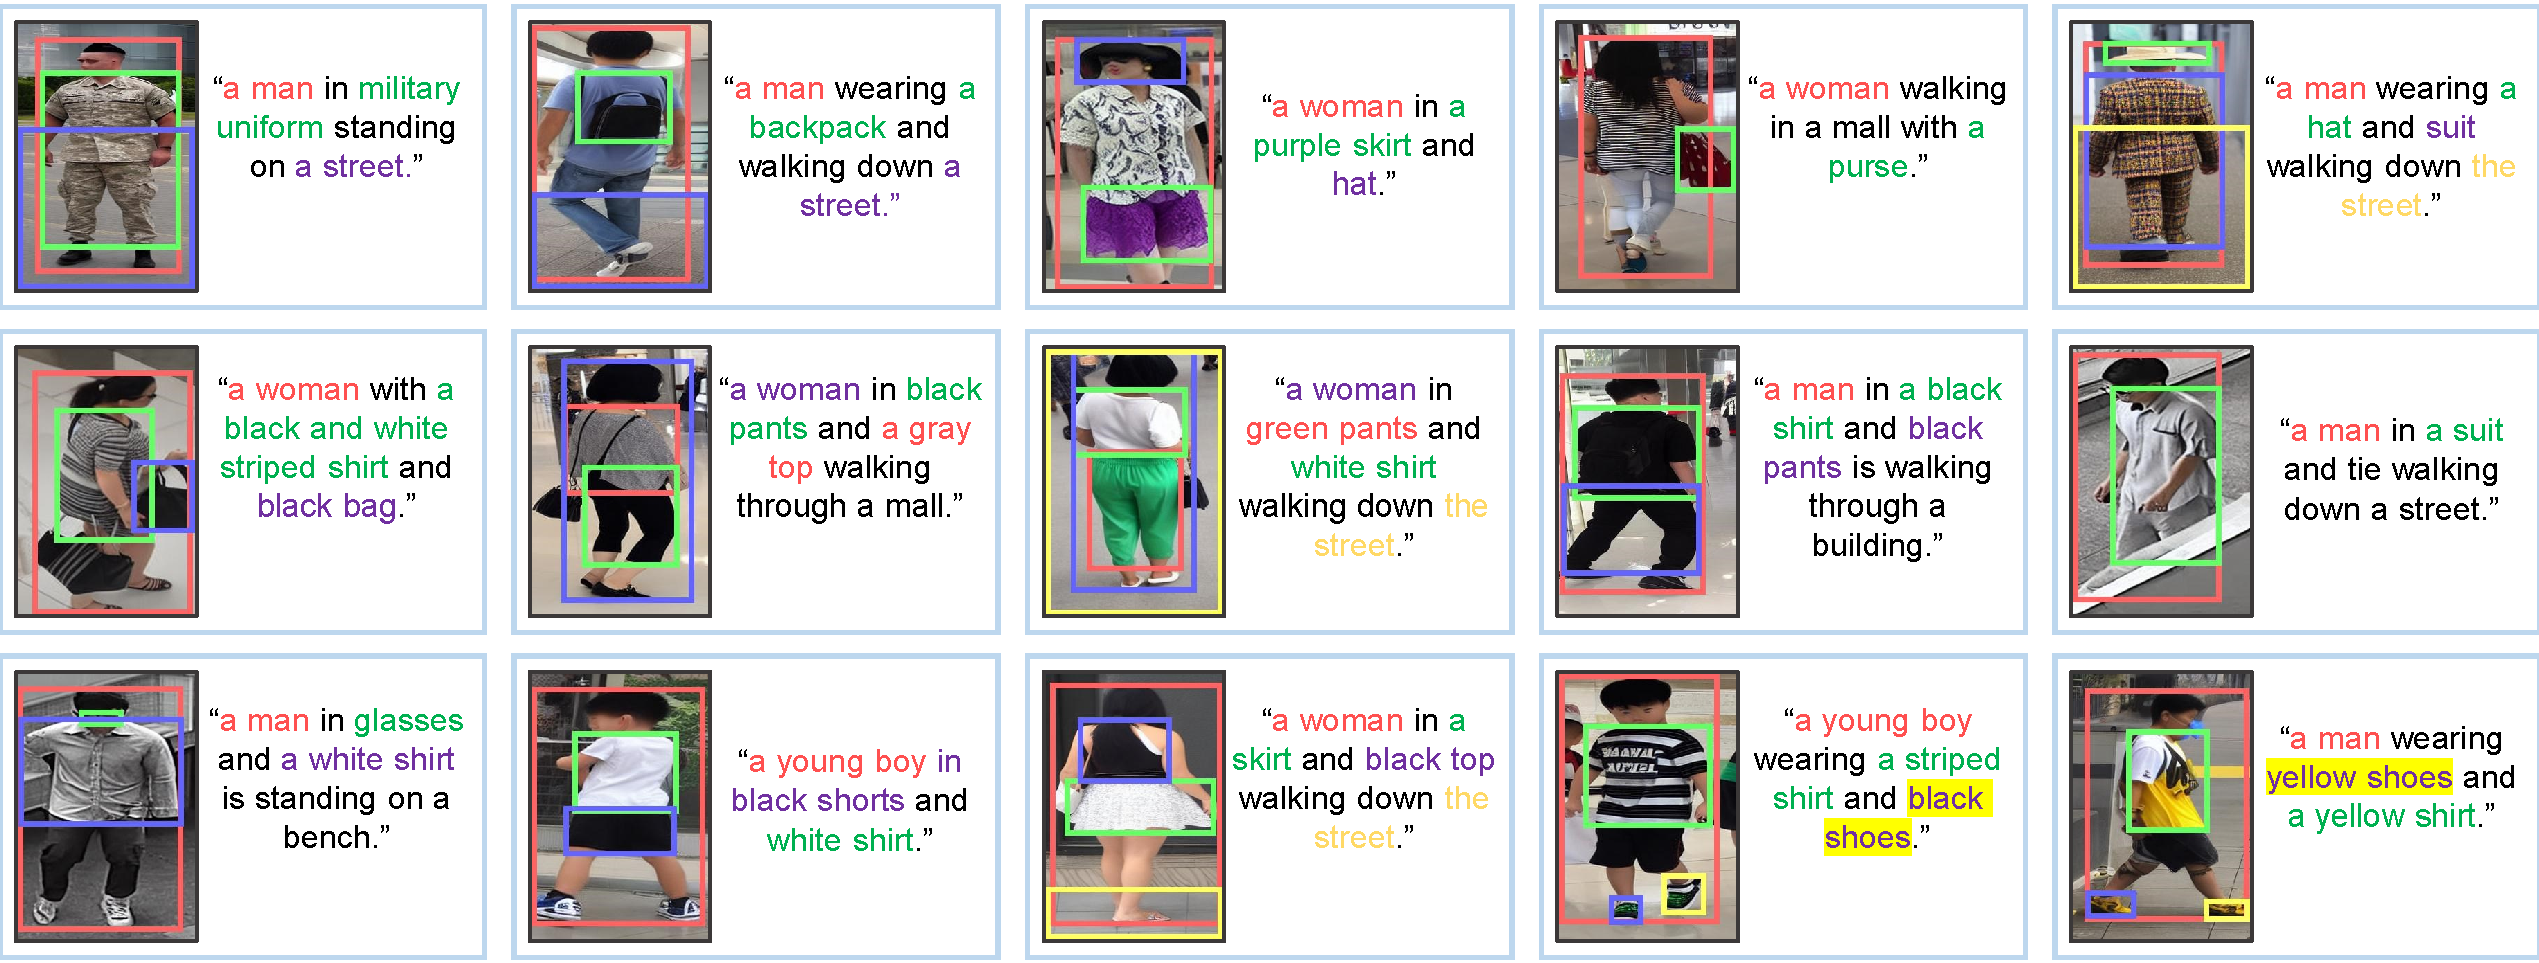
\includegraphics[width=0.92\linewidth]{images/sda.pdf}
\caption{More examples of our proposed SDA. One image-text pair usually carries 2-4 region-phrase annotations.
(Best viewed when zooming in.)}
\label{fig: sda}
\end{figure*}

\subsection{Benchmark Construction} 

\noindent\textbf{Generating Domain-adaptive Images.} 
Providing DaD with suitable textual prompts, the generative model can generate pedestrian images with a style resembling that of the target domain. 
Intuitively, we consider using the text descriptions from the CUHK-PEDES training set as a cue to guide image generation. 
To improve the image diversity, we adopt random seeds in each generation process and perform text adjustments. 
Specifically, given any text in CUHK-PEDES, we leverage EDA~\cite{wei2019eda} for text augmentation, yielding $20$ pieces of different texts (as shown in Fig.~\ref{fig: pipeline}).
EDA encompasses four augmentation techniques: synonym replacement, random insertion, random swap, and random deletion. For each CUHK-PEDES sentence, these four techniques are applied (each with $\alpha=0.5$) to generate five augmented sentences, separately. The resulting 20 texts are then randomly shuffled, and the first 19 augmented sentences are selected. Finally, the original sentence is added to obtain a total of 20 distinct texts.
As a result, $68,126$ CUHK-PEDES texts are converted into 20-fold CUHK-PEDES prompts.
The adjusted CUHK-PEDES prompts are input to generate images. 
Following the above steps, we obtain new domain-adaptive images. 


\noindent\textbf{Image Filtering.} 
To further improve the quality of the generated data, we design some data filtering strategies, as shown in Fig.~\ref{fig: pipeline}.
First, grayscale images are filtered by calculating the mean-variance of the difference between the 3 channels of each picture. 
Next, noise images, which contain distorted portraits, are filtered by OpenPose~\cite{cao2017realtime}.
In Fig.~\ref{fig: bad}, we show some low-quality picture samples.
Although $10.63\%$ of low-quality images are filtered, oversaturation still exists in some of the filtered images due to limitations of the diffusion model itself.


\noindent\textbf{Caption Diversifying.} 
Obtaining high-quality domain-aligned images, we attempt to use the pairs of synthetic images and CUHK-PEDES prompts directly for pretraining. The results are not satisfactory. This limitation arises because every twenty prompts are derived from the same text description, resulting in a lack of textual diversity.
Our solution is to adopt the pretrained Image Captioner model BLIP2 ~\cite{li2023blip} to re-generate the corresponding text descriptions for each synthetic image, yielding new image-text pairs, as shown in Fig.~\ref{fig: pipeline}.
It is worth noting that while BLIP2 provides us with diverse texts, this process may introduce inherent biases present in the BLIP2 model itself.


\noindent\textbf{Region-Phrase Annotation Generation.} 
Many text-based person retrieval works~\cite{shu2022see, yang2023towards, jiang2023cross} have validated that finer-grained features tend to help better image-text alignment. 
Inspired by these works, we further add region annotations to involve multi-granularity visual concepts and corresponding texts. 
Considering the high cost of manual annotation, we employ the Open-set Object Detector Grounding DINO~\cite{liu2023grounding}, which can detect arbitrary objects through human inputs such as category names or reference expressions. 
Specifically, we input image-text pairs into the trained Grounding DINO to obtain region annotations, including bounding boxes, bounding box confidence, and phrase descriptions of the bounding box region.
When Grounding DINO performs the detection, we set both the text threshold and the box threshold to $0.35$.
For each image-text pair, more than two region annotations can be obtained in most cases.


\begin{figure*}[!t]
\centering

\includegraphics[width=1\linewidth]{images/framework.pdf}
\caption{Overview of the proposed Multi-granularity Relation Alignment framework (MRA). MRA first conducts (a) region-phrase encoding and image-text encoding by the shared Vision Encoder ($E_V$) and the shared Text Encoder ($E_T$). The model is constrained with cross-modal alignment at both the (b) region-phrase and (c) image-text levels, where the shared Fusion Encoder ($E_F$) seeks to fuse the vision and text embeddings for the subsequent predictions. 
}
\label{fig: framework}
\end{figure*}


\subsection{Synthetic Domain-Aligned Benchmark} 
\noindent Following the above steps, a large-scale diverse benchmark, \ie, Synthetic Domain-Aligned dataset (SDA), for text-based person retrieval pretraining is built.
In Fig.~\ref{fig: sda}, we show some image-text pairs annotated with region-phrase pairs from SDA. 
The style of SDA images is similar to CUHK-PEDES.
SDA contains $1,217,750$ image-text pairs, roughly $18 \times$ more than the $68,126$ in the CUHK-PEDES training set.
To the best of our knowledge, this is the first pedestrian dataset with region annotations. 
Most of the existing datasets have attribute annotations but provide no information about the location of the relevant attributes in the image.
In SDA, different-grained visual concepts and language description pairs refer to coarse-grained image-text pairs and fine-grained image region-phrase pairs. 
In other terms, an image can contain several different visual concepts, each of which has a corresponding matching textual description, denoted as $(I, T, \{(I_R^i, T_R^i)\}^M_{i=1})$.
$(I, T)$ represents an image-text pair, while $(I_R^i, T_R^i)$ denotes a region-phrase pair.
$I_R^i$ is an image region, which is defined by the bounding box $b^i=(cx, cy, w, h)$. $cx, cy, w, h$ denote the center coordinates, width, and height of the box, respectively. 
When a complete picture represents a visual concept by itself, its bounding box is $(0.5, 0.5, 1, 1)$.
$T_R^i$ is the corresponding textual annotations, \ie, a phrase describing the content of the region $I_R^i$. 
Note that some image-text pairs may not produce region annotations, \ie, $M = 0$. 


\noindent\textbf{Discussion: The contribution to the community.} 
The proposed benchmark follows a similar synthetic manner as existing synthetic pretraining datasets~\cite{yang2023towards,zheng2017unlabeled}, which mitigates the privacy concerns and partially solves the data scarcity for the data-hungry models. 
However, our contribution diverges from these prior works in two significant dimensions: 
\textbf{1) Real-world Image Style.} The visual characteristics of our dataset are meticulously designed to emulate those found in actual pedestrian datasets, thereby promoting effective transfer learning from the pretraining phase to fine-tuning (on real-world data). 
As shown in Section~\ref{experiment}, our approach surpasses APTM~\cite{yang2023towards}, even though it leverages MALS, a more voluminous corpus encompassing $1.51$ million image-text pairs (approximately $0.3$ million more than SDA). 
\textbf{2) Fine-Grained Region-Phrase.} We introduce detailed region-phrase annotations, a critical factor for advancing cross-modal retrieval capabilities and refining the model aptitude for distinguishing subtle visual cues. 
To the best of our knowledge, SDA is one of the pioneering datasets to provide such annotations, whether within the scope of Re-ID or text-based pedestrian retrieval tasks. 
Although some datasets offer attribute information, they often neglect to specify the spatial location of these attributes within the images. 
By offering these precise annotations, SDA empowers researchers to innovate, particularly in improving the model proficiency in recognizing intricate details, thus propelling advancements in fine-grained person retrieval.

